\documentclass[aspectratio=169,11pt]{beamer}

\usetheme{Madrid}
\usecolortheme{default}
\setbeamertemplate{navigation symbols}{}
\setbeamertemplate{footline}[frame number]

\usepackage{amsmath}
\usepackage{amssymb}
\usepackage{booktabs}
\usepackage{graphicx}
\usepackage{array}
\usepackage{tabularx}
\usepackage{multirow}
\usepackage{tikz}
\usepackage{xcolor}
\usepackage[T1]{fontenc}

\usetikzlibrary{arrows.meta,positioning,fit,calc,backgrounds,shapes.geometric,decorations.pathreplacing}

\definecolor{accentblue}{RGB}{37,87,167}
\definecolor{accentred}{RGB}{182,74,54}
\definecolor{accentgold}{RGB}{198,146,53}
\definecolor{softblue}{RGB}{231,239,249}
\definecolor{softred}{RGB}{249,234,229}
\definecolor{softgray}{RGB}{242,243,245}

\setbeamercolor{title}{fg=accentblue}
\setbeamercolor{frametitle}{fg=accentblue}
\setbeamercolor{structure}{fg=accentblue}
\setbeamercolor{block title}{fg=white,bg=accentblue}
\setbeamercolor{block body}{bg=softblue}
\setbeamercolor{alertblock title}{fg=white,bg=accentred}
\setbeamercolor{alertblock body}{bg=softred}

\newcommand{\papersource}{\vspace{0.25em}\hfill{\scriptsize Source: Zhang et al. (2025), \textit{Nature}}}
\newcommand{\sectiondivider}[2]{
  \begin{frame}[plain]
    \vfill
    {\color{accentblue}\LARGE\bfseries #1\par}
    \vspace{0.5em}
    {\large #2\par}
    \vfill
  \end{frame}
}

\title{Shared Neural Dynamics in Social Interaction}
\subtitle{Zhang et al. (2025), \textit{Inter-brain neural dynamics in biological and artificial intelligence systems}}
\author{Neuroeconomics Class Presentation Draft}
\institute{Nature, 645, 991--1001}
\date{May 2026}

\begin{document}

\frame{\titlepage}

\begin{frame}{Roadmap}
\small
\tableofcontents[hideallsubsections]
\end{frame}

\section{Opening}
\sectiondivider{Opening}{Why this paper matters for neuroeconomics}

\begin{frame}{One-sentence thesis}
\begin{alertblock}{Core idea}
Social decision-making may not live entirely inside one brain. During interaction, two agents may form a coupled neural system with measurable \textbf{shared neural dynamics}.
\end{alertblock}
\vspace{0.4em}
\begin{itemize}
  \item The paper studies both \textbf{freely interacting mice} and \textbf{interacting AI agents}.
  \item The authors ask whether social interaction creates a real \textbf{shared neural structure}, not just matching sensory input or matching movement.
  \item That question is deeply neuroeconomic because many decisions are \textbf{strategic, reciprocal, and interdependent}.
\end{itemize}
\end{frame}

\begin{frame}{Why this belongs in neuroeconomics}
\begin{columns}[T]
  \begin{column}{0.48\textwidth}
    \begin{block}{Standard framing}
    \begin{itemize}
      \item How does one brain process a social cue?
      \item How does one individual make a decision?
      \item The partner is often treated like the environment.
    \end{itemize}
    \end{block}
  \end{column}
  \begin{column}{0.48\textwidth}
    \begin{block}{This paper's framing}
    \begin{itemize}
      \item Two interacting agents form a feedback loop.
      \item My action changes your state, and your response changes mine.
      \item Neural activity may also become coupled across agents.
    \end{itemize}
    \end{block}
  \end{column}
\end{columns}
\vspace{0.2em}
\begin{center}
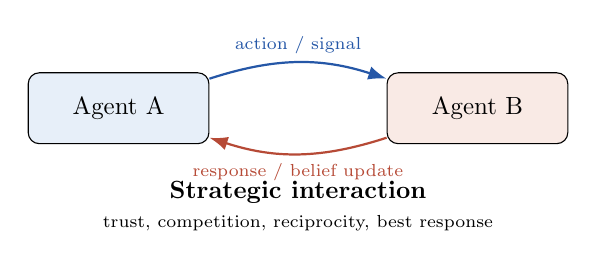
\begin{tikzpicture}[>=Latex, node distance=1.25cm, scale=0.9, transform shape]
  \node[draw, rounded corners, fill=softblue, minimum width=2.55cm, minimum height=1.0cm] (a) {Agent A};
  \node[draw, rounded corners, fill=softred, right=2.5cm of a, minimum width=2.55cm, minimum height=1.0cm] (b) {Agent B};
  \draw[->, thick, accentblue] (a) to[bend left=18] node[above] {\scriptsize action / signal} (b);
  \draw[->, thick, accentred] (b) to[bend left=18] node[below] {\scriptsize response / belief update} (a);
  \node[below=0.9cm of $(a)!0.5!(b)$, align=center] {\textbf{Strategic interaction} \\ \scriptsize trust, competition, reciprocity, best response};
\end{tikzpicture}
\end{center}
\end{frame}

\begin{frame}{Paper in plain English}
\begin{block}{Main question}
When two individuals interact, do their brains develop a measurable \textbf{shared neural subspace} that cannot be reduced to the same stimulus or the same action?
\end{block}
\vspace{0.3em}
\begin{itemize}
  \item Biological side: simultaneous dmPFC calcium imaging in two mice.
  \item Artificial side: internal RNN activity in two multi-agent RL systems.
  \item Big ambition: move from \textbf{single-brain social neuroscience} to \textbf{multi-brain systems neuroscience}.
\end{itemize}
\end{frame}

\begin{frame}{The paper's logic}
\begin{center}
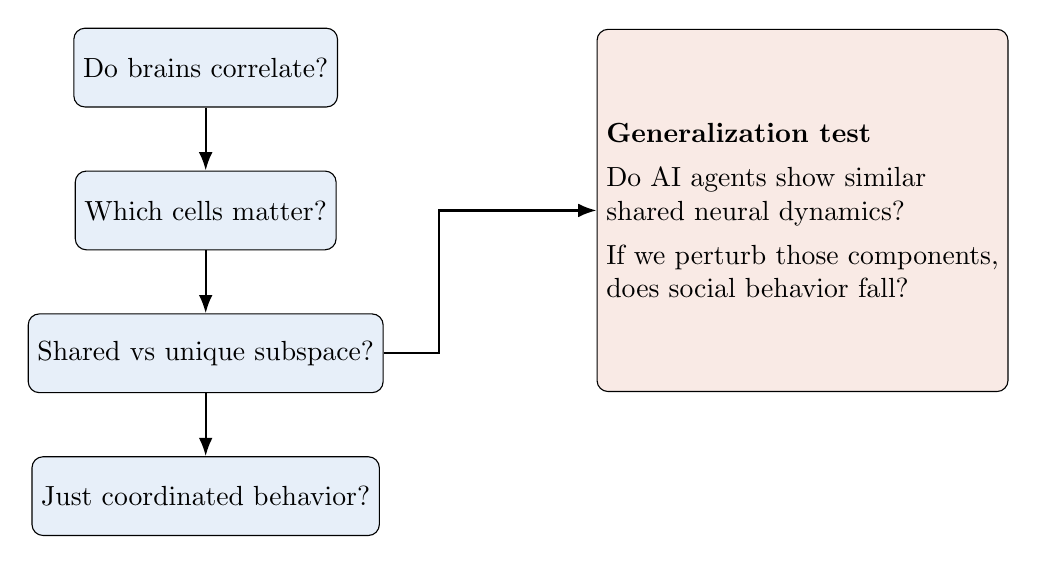
\begin{tikzpicture}[>=Latex, node distance=0.8cm]
  \node[draw, rounded corners, fill=softblue, minimum width=3.0cm, minimum height=1.0cm] (q1) {Do brains correlate?};
  \node[draw, rounded corners, fill=softblue, below=of q1, minimum width=3.0cm, minimum height=1.0cm] (q2) {Which cells matter?};
  \node[draw, rounded corners, fill=softblue, below=of q2, minimum width=3.0cm, minimum height=1.0cm] (q3) {Shared vs unique subspace?};
  \node[draw, rounded corners, fill=softblue, below=of q3, minimum width=3.0cm, minimum height=1.0cm] (q4) {Just coordinated behavior?};
  \node[draw, rounded corners, fill=softred, right=3.3cm of q2, minimum width=4.5cm, minimum height=4.6cm, align=left] (q5) {
    \textbf{Generalization test}\\[0.4em]
    Do AI agents show similar\\
    shared neural dynamics?\\[0.4em]
    If we perturb those components,\\
    does social behavior fall?
  };
  \draw[->, thick] (q1) -- (q2);
  \draw[->, thick] (q2) -- (q3);
  \draw[->, thick] (q3) -- (q4);
  \draw[->, thick] (q3.east) -- ++(0.7,0) |- (q5.west);
\end{tikzpicture}
\end{center}
\end{frame}

\begin{frame}{What this presentation will do}
\begin{enumerate}
  \item Clarify the \textbf{research question} and the alternative explanations the paper tries to rule out
  \item Walk through the \textbf{experimental design} in mice and AI
  \item Organize the \textbf{main results} into a clean story
  \item Evaluate the authors' \textbf{interpretation}
  \item Explain whether I am \textbf{convinced}
  \item Propose a \textbf{better design} and a \textbf{new neuroeconomics-style extension}
\end{enumerate}
\end{frame}

\section{Design}
\sectiondivider{Design}{What exactly did the authors do?}

\begin{frame}{Two systems, one analytical idea}
\begin{columns}[T]
  \begin{column}{0.49\textwidth}
    \begin{block}{Biological system}
    \begin{itemize}
      \item Two freely interacting mice
      \item Simultaneous dmPFC calcium imaging
      \item Comparison of \textbf{glutamatergic} and \textbf{GABAergic} neurons
      \item Interaction, separation, shuffled, and cross-pair controls
    \end{itemize}
    \end{block}
  \end{column}
  \begin{column}{0.49\textwidth}
    \begin{block}{Artificial system}
    \begin{itemize}
      \item Two MARL agents learning to interact
      \item Analysis of internal RNN activations
      \item Comparison of \textbf{social} and \textbf{non-social} training
      \item Direct perturbation of shared components
    \end{itemize}
    \end{block}
  \end{column}
\end{columns}
\vspace{0.3em}
\begin{center}
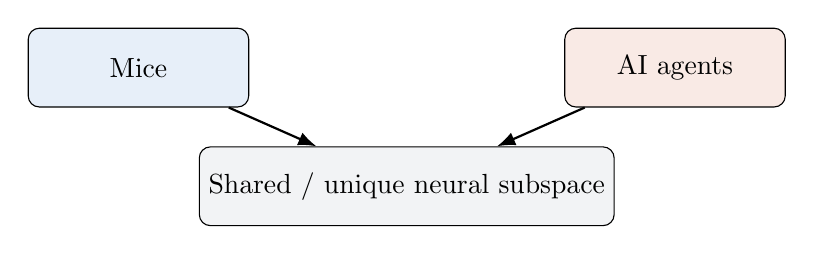
\begin{tikzpicture}[>=Latex, node distance=1.2cm]
  \node[draw, rounded corners, fill=softblue, minimum width=2.8cm, minimum height=1.0cm] (mice) {Mice};
  \node[draw, rounded corners, fill=softred, right=4.0cm of mice, minimum width=2.8cm, minimum height=1.0cm] (ai) {AI agents};
  \node[draw, rounded corners, fill=softgray, below=1.0cm of $(mice)!0.5!(ai)$, minimum width=4.6cm, minimum height=1.0cm] (analysis) {Shared / unique neural subspace};
  \draw[->, thick] (mice) -- (analysis);
  \draw[->, thick] (ai) -- (analysis);
\end{tikzpicture}
\end{center}
\end{frame}

\begin{frame}{Mouse dataset at a glance}
\begin{columns}[T]
  \begin{column}{0.56\textwidth}
    \begin{itemize}
      \item Brain region: \textbf{dmPFC}, a region linked to social information and social behavior regulation.
      \item Recording method: \textbf{in vivo microendoscopic calcium imaging}.
      \item Cell-type-specific recording:
      \begin{itemize}
        \item CaMKII-positive glutamatergic neurons
        \item mDLX-positive GABAergic neurons
      \end{itemize}
      \item The interactions are naturalistic rather than tightly scripted trial-by-trial events.
    \end{itemize}
  \end{column}
  \begin{column}{0.42\textwidth}
    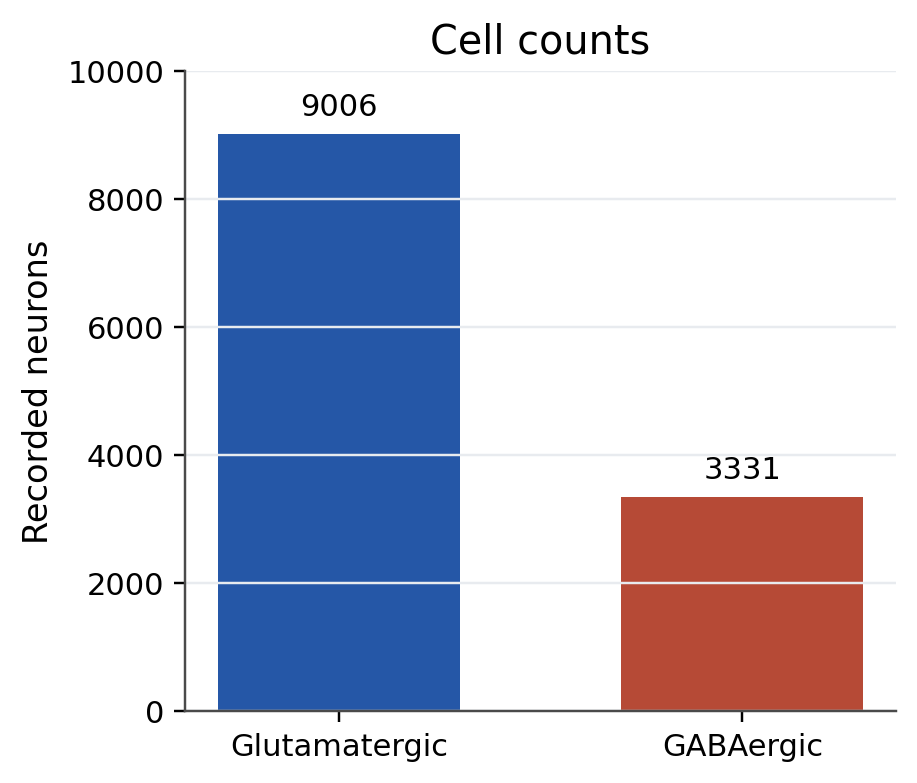
\includegraphics[width=\linewidth]{figures/cell_counts.png}
  \end{column}
\end{columns}
\papersource
\end{frame}

\begin{frame}{Behavioral conditions and controls}
\begin{columns}[T]
  \begin{column}{0.48\textwidth}
    \begin{block}{Main condition}
    \begin{itemize}
      \item \textbf{Interaction session}: two mice freely interact
      \item Social and non-social actions unfold naturally
    \end{itemize}
    \end{block}
    \begin{block}{Control conditions}
    \begin{itemize}
      \item \textbf{Separation}: a physical divider blocks direct interaction
      \item \textbf{Phase-randomized}: temporal phase is scrambled
      \item \textbf{Cross-pair}: signals are compared across mice that never interacted
    \end{itemize}
    \end{block}
  \end{column}
  \begin{column}{0.48\textwidth}
    \begin{alertblock}{What each control tests}
    \begin{itemize}
      \item Separation: not every shared environment creates coupling
      \item Phase-randomized: not a simple autocorrelation artifact
      \item Cross-pair: not any arbitrary pair of animals
    \end{itemize}
    \end{alertblock}
  \end{column}
\end{columns}
\end{frame}

\begin{frame}{Behavioral annotation was broad}
\begin{columns}[T]
  \begin{column}{0.48\textwidth}
    \begin{block}{Social behaviors}
    \scriptsize
    attack, tussle, chase, threaten, escape, defend, flinch,\\
    general sniff, face sniff, genital sniff, approach, follow
    \end{block}
  \end{column}
  \begin{column}{0.48\textwidth}
    \begin{block}{Non-social behaviors}
    \scriptsize
    dig, self grooming, climb, explore object, bite object, stand
    \end{block}
  \end{column}
\end{columns}
\vspace{0.6em}
\begin{block}{Why that matters}
The goal is not just to ask whether the mice are ``being social.'' The authors want to distinguish:
\begin{itemize}
  \item which kinds of interaction produce stronger cross-brain coupling,
  \item whether non-social activity lives more in the unique subspace,
  \item and whether complementary actions such as \textit{attack} versus \textit{escape} matter more than identical actions.
\end{itemize}
\end{block}
\end{frame}

\begin{frame}{Why compare GABAergic and glutamatergic neurons?}
\begin{columns}[T]
  \begin{column}{0.46\textwidth}
    \begin{block}{Initial expectation}
    Since glutamatergic neurons dominate the cortex numerically, one could expect them to drive most population-level inter-brain correlation.
    \end{block}
  \end{column}
  \begin{column}{0.50\textwidth}
    \begin{alertblock}{What the paper finds}
    The stronger social coupling appears in \textbf{GABAergic neurons}, not in the larger glutamatergic population.
    \end{alertblock}
  \end{column}
\end{columns}
\vspace{0.4em}
\begin{center}
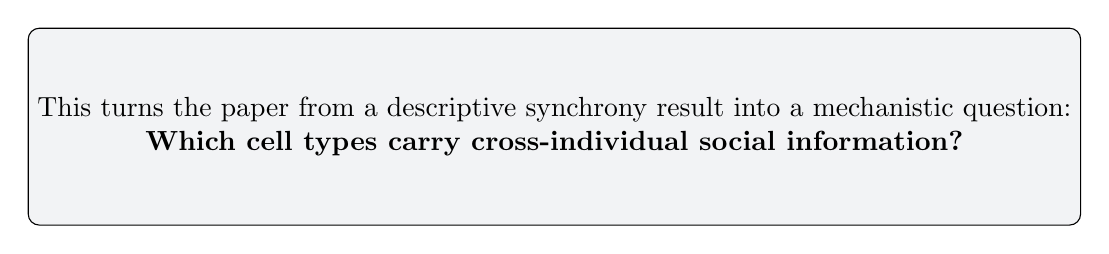
\begin{tikzpicture}[>=Latex]
  \node[draw, rounded corners, fill=softgray, minimum width=11.4cm, minimum height=2.5cm, align=center] (box) {
    This turns the paper from a descriptive synchrony result into a mechanistic question:\\
    \textbf{Which cell types carry cross-individual social information?}
  };
\end{tikzpicture}
\end{center}
\end{frame}

\begin{frame}{AI task design in one slide}
\begin{columns}[T]
  \begin{column}{0.55\textwidth}
    \begin{itemize}
      \item Two agents: \textbf{chaser} and \textbf{explorer}
      \item Multi-agent reinforcement learning
      \item Each agent uses an \textbf{actor-critic architecture with a 256-unit RNN}
      \item \textbf{Social task}: partner-relevant reward and partner in vision
      \item \textbf{Non-social task}: social reward removed, interaction no longer behaviorally useful
    \end{itemize}
  \end{column}
  \begin{column}{0.41\textwidth}
    \begin{center}
    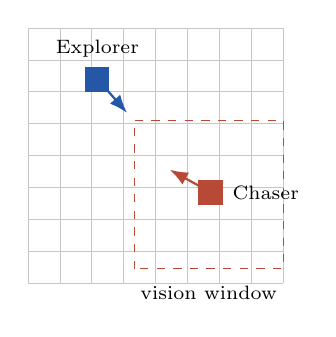
\begin{tikzpicture}[>=Latex, scale=0.9]
      \draw[step=0.45cm, gray!45, very thin] (0,0) grid (3.6,3.6);
      \fill[accentblue] (0.8,2.7) rectangle +(0.35,0.35);
      \fill[accentred] (2.4,1.1) rectangle +(0.35,0.35);
      \draw[accentred, thick, ->] (2.58,1.28) -- (2.0,1.6);
      \draw[accentblue, thick, ->] (0.98,2.88) -- (1.4,2.4);
      \node[above] at (0.98,3.05) {\scriptsize Explorer};
      \node[right] at (2.75,1.28) {\scriptsize Chaser};
      \draw[dashed, accentred] (1.5,0.2) rectangle (3.6,2.3);
      \node[below] at (2.55,0.1) {\scriptsize vision window};
    \end{tikzpicture}
    \end{center}
  \end{column}
\end{columns}
\papersource
\end{frame}

\begin{frame}{Why put mice and AI in the same paper?}
\begin{columns}[T]
  \begin{column}{0.48\textwidth}
    \begin{block}{Mouse side gives}
    \begin{itemize}
      \item biological realism
      \item cell-type specificity
      \item natural social interaction
    \end{itemize}
    \end{block}
  \end{column}
  \begin{column}{0.48\textwidth}
    \begin{block}{AI side gives}
    \begin{itemize}
      \item full access to internal states
      \item cleaner control over rewards and inputs
      \item direct perturbation of the shared components
    \end{itemize}
    \end{block}
  \end{column}
\end{columns}
\vspace{0.4em}
\begin{alertblock}{Combined logic}
If shared neural dynamics appear in both systems, and perturbing them reduces social behavior in AI, the authors can argue for a more general principle of interacting intelligence.
\end{alertblock}
\end{frame}

\section{Methods}
\sectiondivider{Methods}{How do they define ``shared''?}

\begin{frame}{Method map}
\begin{center}
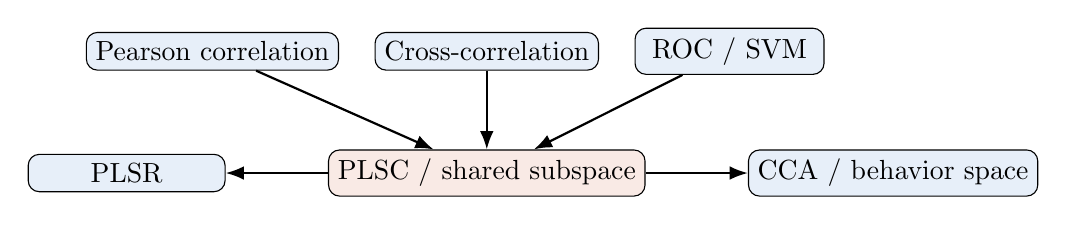
\begin{tikzpicture}[>=Latex, node distance=0.95cm]
  \node[draw, rounded corners, fill=softblue, minimum width=2.3cm] (m1) {Pearson correlation};
  \node[draw, rounded corners, fill=softblue, right=0.45cm of m1, minimum width=2.4cm] (m2) {Cross-correlation};
  \node[draw, rounded corners, fill=softblue, right=0.45cm of m2, minimum width=2.4cm] (m3) {ROC / SVM};
  \node[draw, rounded corners, fill=softred, below=1.0cm of m2, minimum width=3.1cm] (m4) {PLSC / shared subspace};
  \node[draw, rounded corners, fill=softblue, left=1.3cm of m4, minimum width=2.5cm] (m5) {PLSR};
  \node[draw, rounded corners, fill=softblue, right=1.3cm of m4, minimum width=2.5cm] (m6) {CCA / behavior space};
  \draw[->, thick] (m1) -- (m4);
  \draw[->, thick] (m2) -- (m4);
  \draw[->, thick] (m3) -- (m4);
  \draw[->, thick] (m4) -- (m5);
  \draw[->, thick] (m4) -- (m6);
\end{tikzpicture}
\end{center}
\vspace{0.5em}
\begin{itemize}
  \item The first tools test whether cross-brain coupling exists at all.
  \item PLSC is the conceptual center of the paper.
  \item PLSR and CCA ask what kinds of behavior actually explain the shared structure.
\end{itemize}
\end{frame}

\begin{frame}{Pearson correlation and cross-correlation}
\begin{columns}[T]
  \begin{column}{0.48\textwidth}
    \begin{block}{Pearson correlation}
    Measure whether aggregate activity in two brains rises and falls together.
    \end{block}
    \begin{block}{Question answered}
    Is there inter-brain coupling above chance?
    \end{block}
  \end{column}
  \begin{column}{0.48\textwidth}
    \begin{block}{Cross-correlation}
    Evaluate correlation across different time lags.
    \end{block}
    \begin{block}{Question answered}
    If the peak is near 0 s, the coupling is close to synchronous rather than delayed noise.
    \end{block}
  \end{column}
\end{columns}
\vspace{0.4em}
\begin{alertblock}{Why the controls matter}
When phase randomization destroys the peak, the original cross-brain signal is unlikely to be just a by-product of one signal's internal temporal smoothness.
\end{alertblock}
\end{frame}

\begin{frame}{PLSC intuition}
\begin{columns}[T]
  \begin{column}{0.55\textwidth}
    \begin{itemize}
      \item Each mouse has a high-dimensional neural activity space.
      \item PLSC finds the dimensions that \textbf{co-vary most strongly across the two brains}.
      \item This is not neuron-to-neuron matching. It is pattern-to-pattern matching.
    \end{itemize}
    \begin{block}{Output}
    \textbf{Shared neural dimensions} and \textbf{unique neural dimensions}
    \end{block}
  \end{column}
  \begin{column}{0.41\textwidth}
    \begin{center}
    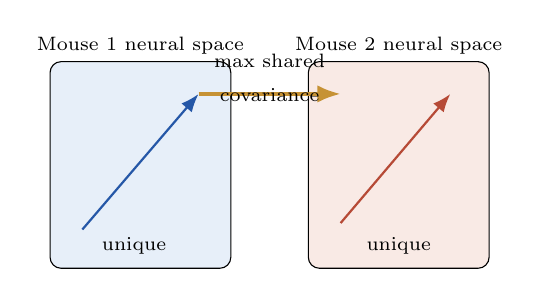
\begin{tikzpicture}[>=Latex, scale=0.82]
      \draw[rounded corners, fill=softblue] (0,0) rectangle (2.8,3.2);
      \draw[rounded corners, fill=softred] (4.0,0) rectangle (6.8,3.2);
      \draw[thick, accentblue, ->] (0.5,0.6) -- (2.3,2.7);
      \draw[thick, accentred, ->] (4.5,0.7) -- (6.2,2.7);
      \draw[very thick, accentgold, ->] (2.3,2.7) -- (4.5,2.7);
      \node at (1.4,3.45) {\scriptsize Mouse 1 neural space};
      \node at (5.4,3.45) {\scriptsize Mouse 2 neural space};
      \node[align=center] at (3.4,2.95) {\scriptsize max shared\\ \scriptsize covariance};
      \node[align=center] at (1.3,0.35) {\scriptsize unique};
      \node[align=center] at (5.4,0.35) {\scriptsize unique};
    \end{tikzpicture}
    \end{center}
  \end{column}
\end{columns}
\end{frame}

\begin{frame}{Shared subspace versus unique subspace}
\begin{columns}[T]
  \begin{column}{0.49\textwidth}
    \begin{block}{Shared neural subspace}
    \begin{itemize}
      \item Activity that changes across both individuals
      \item More strongly linked to social interaction
      \item Can contain information about both self and partner
    \end{itemize}
    \end{block}
  \end{column}
  \begin{column}{0.49\textwidth}
    \begin{block}{Unique neural subspace}
    \begin{itemize}
      \item Activity specific to one individual
      \item More strongly linked to non-social or self-specific behavior
      \item Less tied to the partner's moment-to-moment state
    \end{itemize}
    \end{block}
  \end{column}
\end{columns}
\vspace{0.4em}
\begin{center}
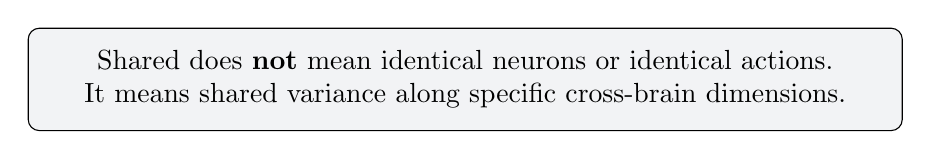
\begin{tikzpicture}[>=Latex]
  \node[draw, rounded corners, fill=softgray, minimum width=11.1cm, minimum height=1.3cm, align=center] {
    Shared does \textbf{not} mean identical neurons or identical actions.\\
    It means shared variance along specific cross-brain dimensions.
  };
\end{tikzpicture}
\end{center}
\end{frame}

\begin{frame}{Behavioral subspace analysis}
\begin{columns}[T]
  \begin{column}{0.46\textwidth}
    \begin{block}{Coordinated behavioral subspace}
    The part of behavior that changes together across both mice.
    \end{block}
    \begin{block}{Uncoordinated behavioral subspace}
    Different actions that are still linked inside the same interaction.
    \end{block}
  \end{column}
  \begin{column}{0.50\textwidth}
    \begin{center}
    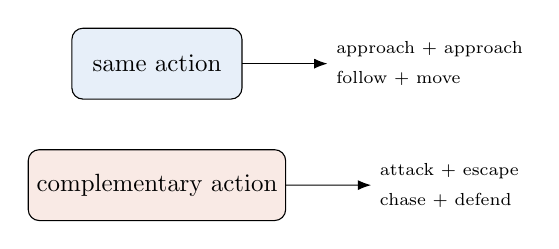
\begin{tikzpicture}[>=Latex, scale=0.9, transform shape]
      \node[draw, rounded corners, fill=softblue, minimum width=2.4cm, minimum height=1cm] (same) {same action};
      \node[draw, rounded corners, fill=softred, below=0.7cm of same, minimum width=2.4cm, minimum height=1cm] (comp) {complementary action};
      \node[right=1.2cm of same, align=left] (text1) {\scriptsize approach + approach\\ \scriptsize follow + move};
      \node[right=1.2cm of comp, align=left] (text2) {\scriptsize attack + escape\\ \scriptsize chase + defend};
      \draw[->] (same) -- (text1);
      \draw[->] (comp) -- (text2);
    \end{tikzpicture}
    \end{center}
  \end{column}
\end{columns}
\vspace{0.4em}
\begin{alertblock}{Critical interpretation test}
If the shared neural subspace can be explained entirely by coordinated behavior, then the paper's big claim about a coupled social system becomes much weaker.
\end{alertblock}
\end{frame}

\begin{frame}{Why the AI analysis is methodologically important}
\begin{itemize}
  \item In mice, the paper mainly provides recording, decoding, and subspace analyses.
  \item In AI, the authors can ask a stronger causal question:
\end{itemize}
\begin{center}
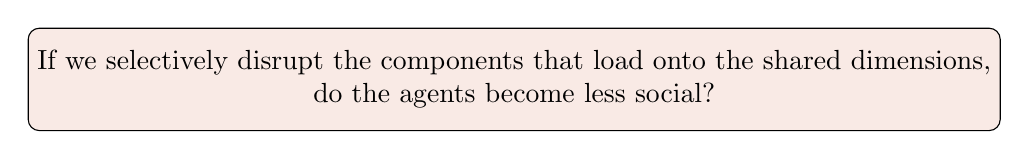
\begin{tikzpicture}[>=Latex]
  \node[draw, rounded corners, fill=softred, minimum width=9.7cm, minimum height=1.3cm, align=center] {
    If we selectively disrupt the components that load onto the shared dimensions,\\
    do the agents become less social?
  };
\end{tikzpicture}
\end{center}
\vspace{0.4em}
\begin{itemize}
  \item That is the paper's clearest evidence for \textbf{functional relevance}.
\end{itemize}
\end{frame}

\section{MouseResults}
\sectiondivider{Mouse Results}{What do we learn from real brains?}

\begin{frame}{Result roadmap: mice}
\begin{enumerate}
  \item Inter-brain correlation appears during interaction
  \item GABAergic neurons are more socially coupled than glutamatergic neurons
  \item Neural activity splits into shared and unique subspaces
  \item The shared subspace is more social than the unique subspace
  \item Shared dynamics are not reducible to simple coordinated movement
\end{enumerate}
\end{frame}

\begin{frame}{Result 1: inter-brain correlation exists}
\begin{block}{Main finding}
During \textbf{interaction sessions}, the two mice show significant dmPFC coupling. That coupling is reduced or absent in \textbf{separation}, \textbf{cross-pair}, and \textbf{phase-randomized} controls.
\end{block}
\vspace{0.5em}
\begin{columns}[T]
  \begin{column}{0.56\textwidth}
    \begin{itemize}
      \item The cross-correlation peak is near 0 s.
      \item The signal survives pre-whitening.
      \item This makes a simple autocorrelation explanation less plausible.
    \end{itemize}
  \end{column}
  \begin{column}{0.40\textwidth}
    \begin{center}
    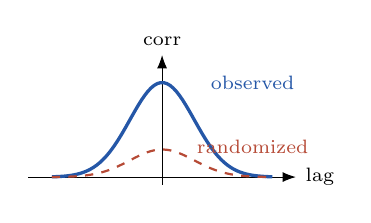
\begin{tikzpicture}[>=Latex]
      \draw[->] (-1.7,0) -- (1.7,0) node[right] {\scriptsize lag};
      \draw[->] (0,-0.1) -- (0,1.55) node[above] {\scriptsize corr};
      \draw[accentblue, very thick, domain=-1.4:1.4, samples=70] plot (\x,{1.2*exp(-3*\x*\x)});
      \draw[accentred, thick, dashed, domain=-1.4:1.4, samples=70] plot (\x,{0.35*exp(-3*\x*\x)});
      \node[accentblue] at (1.15,1.2) {\scriptsize observed};
      \node[accentred] at (1.15,0.38) {\scriptsize randomized};
    \end{tikzpicture}
    \end{center}
  \end{column}
\end{columns}
\papersource
\end{frame}

\begin{frame}{Why this already matters for neuroeconomics}
\begin{columns}[T]
  \begin{column}{0.48\textwidth}
    \begin{block}{Economic intuition}
    In strategic interaction, choices are not independent draws.
    \end{block}
    \begin{itemize}
      \item My best response depends on your move.
      \item Your move depends on what you expect from me.
    \end{itemize}
  \end{column}
  \begin{column}{0.48\textwidth}
    \begin{block}{Neural translation}
    Inter-brain coupling suggests that neural states may also become interdependent rather than remaining isolated optimization problems.
    \end{block}
  \end{column}
\end{columns}
\end{frame}

\begin{frame}{Result 2: GABAergic neurons are more socially coupled}
\begin{columns}[T]
  \begin{column}{0.50\textwidth}
    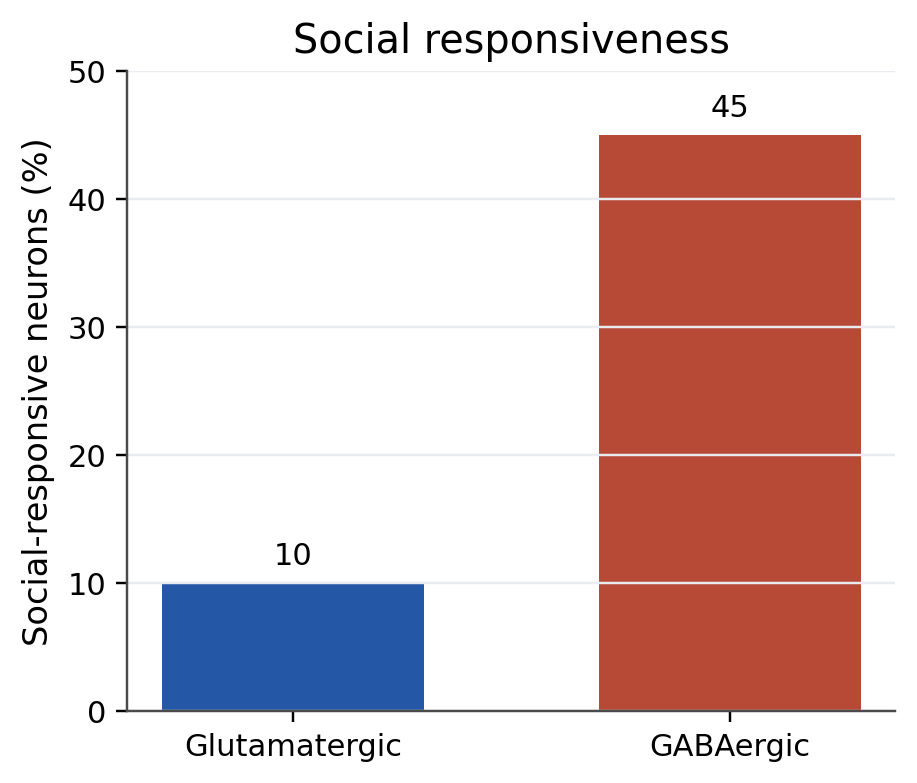
\includegraphics[width=\linewidth]{figures/social_responsiveness.png}
  \end{column}
  \begin{column}{0.46\textwidth}
    \begin{itemize}
      \item About \textbf{45\%} of GABAergic neurons are responsive to social interaction.
      \item Only about \textbf{10\%} of glutamatergic neurons are.
      \item GABAergic populations also decode social behaviors better.
      \item The effect is not explained by firing-rate differences.
    \end{itemize}
  \end{column}
\end{columns}
\papersource
\end{frame}

\begin{frame}{Result 2b: decoding evidence points in the same direction}
\begin{columns}[T]
  \begin{column}{0.52\textwidth}
    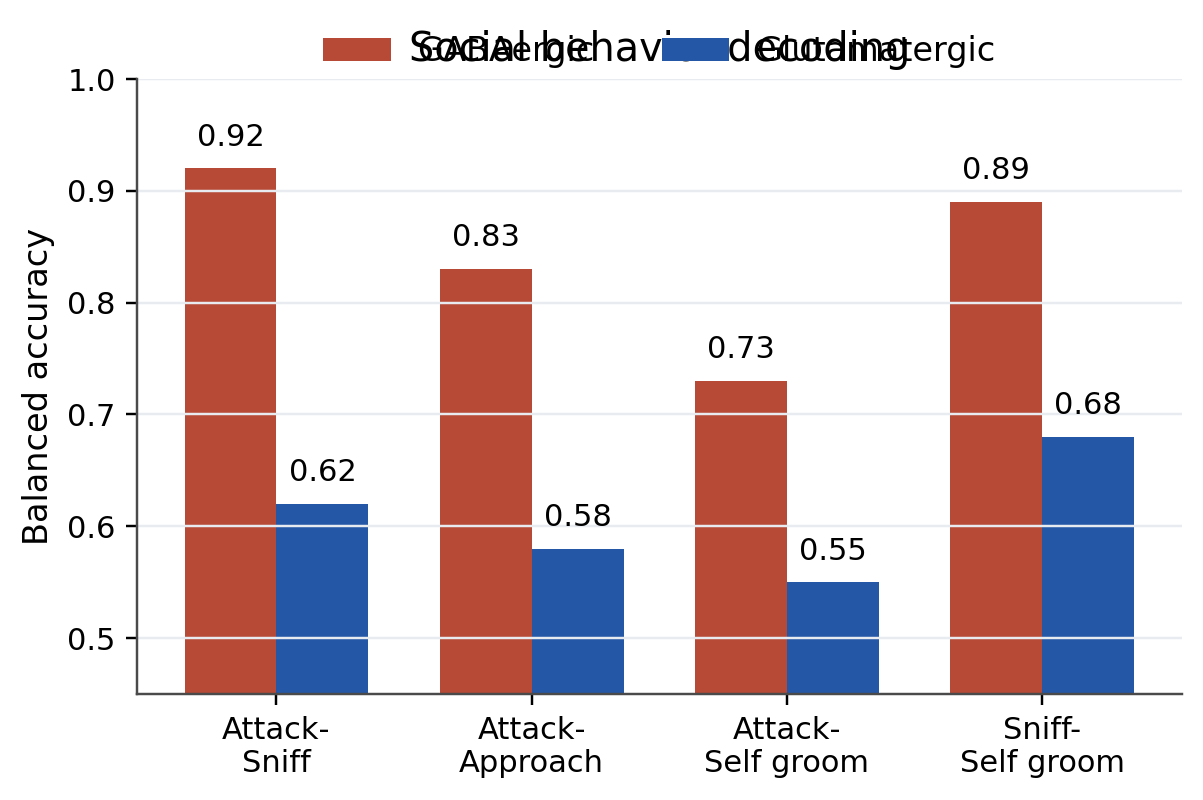
\includegraphics[width=\linewidth]{figures/decoding_summary.png}
  \end{column}
  \begin{column}{0.42\textwidth}
    \begin{alertblock}{Interpretation}
    GABAergic neurons are not just more correlated. They also carry richer information about social events.
    \end{alertblock}
    \vspace{0.3em}
    \begin{itemize}
      \item Better social versus social classification
      \item Better social versus self-groom classification
      \item More consistent with interaction-state tracking
    \end{itemize}
  \end{column}
\end{columns}
\vspace{0.1em}
{\scriptsize Note: bars summarize the direction and relative magnitude of the SVM decoding comparisons reported in Fig. 1q--t.}
\end{frame}

\begin{frame}{Result 3: not all GABAergic neurons matter equally}
\begin{columns}[T]
  \begin{column}{0.46\textwidth}
    \begin{block}{Computational removal analysis}
    Removing \textbf{social-responsive} GABAergic neurons causes a clear drop in inter-brain correlation.
    \end{block}
    \begin{itemize}
      \item Removing non-social-responsive GABAergic neurons does not do the same
      \item Similar removals in glutamatergic populations have weaker effects
    \end{itemize}
  \end{column}
  \begin{column}{0.50\textwidth}
    \begin{center}
    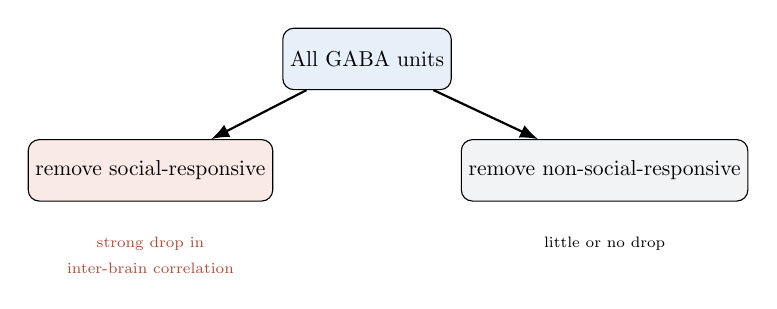
\begin{tikzpicture}[>=Latex, scale=0.78, transform shape]
      \node[draw, rounded corners, fill=softblue, minimum width=2.7cm, minimum height=1.0cm] (all) {All GABA units};
      \node[draw, rounded corners, fill=softred, below left=0.8cm and 0.15cm of all, minimum width=2.45cm, minimum height=1.0cm] (social) {remove social-responsive};
      \node[draw, rounded corners, fill=softgray, below right=0.8cm and 0.15cm of all, minimum width=2.45cm, minimum height=1.0cm] (nonsocial) {remove non-social-responsive};
      \draw[->, thick] (all) -- (social);
      \draw[->, thick] (all) -- (nonsocial);
      \node[below=0.45cm of social, align=center, accentred] {\scriptsize strong drop in\\ \scriptsize inter-brain correlation};
      \node[below=0.45cm of nonsocial, align=center] {\scriptsize little or no drop};
    \end{tikzpicture}
    \end{center}
  \end{column}
\end{columns}
\end{frame}

\begin{frame}{Result 4: neural activity splits into shared and unique parts}
\begin{columns}[T]
  \begin{column}{0.48\textwidth}
    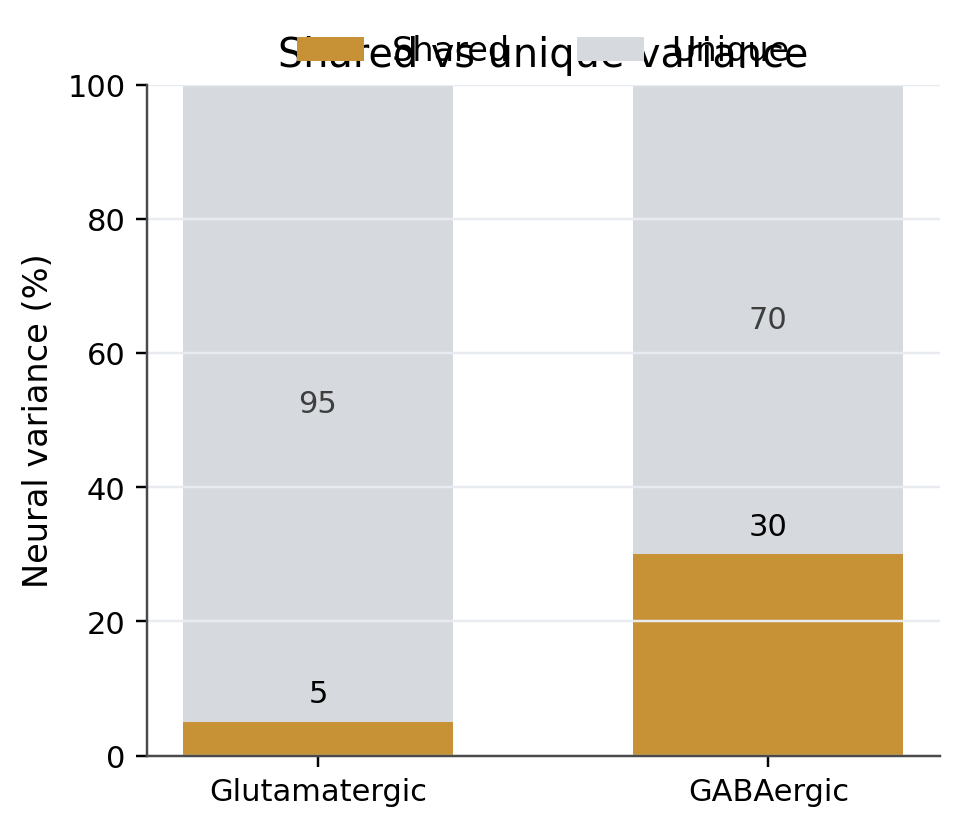
\includegraphics[width=0.84\linewidth]{figures/shared_unique_variance.png}
  \end{column}
  \begin{column}{0.46\textwidth}
    \begin{itemize}
      \item Significant shared dimensions appear during live interaction.
      \item They are nearly absent in separation.
      \item GABAergic populations have about \textbf{30\%} shared variance.
      \item Glutamatergic populations have only about \textbf{5\%}.
    \end{itemize}
    \begin{alertblock}{Key message}
    The gap is not just stronger average synchrony. Much more of the GABAergic neural space changes jointly across the two animals.
    \end{alertblock}
  \end{column}
\end{columns}
\papersource
\end{frame}

\begin{frame}{Result 4b: the top shared dimension is already much stronger}
\begin{columns}[T]
  \begin{column}{0.52\textwidth}
    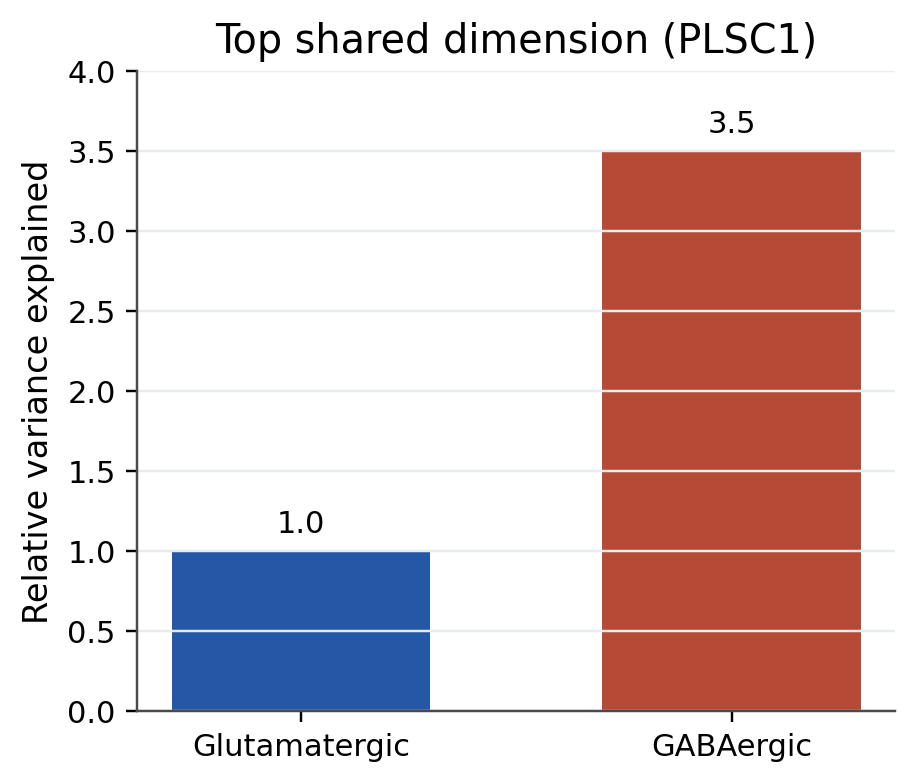
\includegraphics[width=\linewidth]{figures/top_dimension.png}
  \end{column}
  \begin{column}{0.42\textwidth}
    \begin{itemize}
      \item The paper reports that GABAergic PLSC1 explains about \textbf{3.5 times} as much variance as glutamatergic PLSC1.
      \item So the difference is not only about having more shared dimensions.
      \item The leading shared dimension itself is stronger.
    \end{itemize}
  \end{column}
\end{columns}
\end{frame}

\begin{frame}{Result 5: the shared subspace is more social}
\begin{columns}[T]
  \begin{column}{0.54\textwidth}
    \begin{itemize}
      \item The authors use PLSR to explain neural subspaces with behavior.
      \item \textbf{Social behaviors} explain more variance in the shared subspace.
      \item \textbf{Non-social behaviors} explain more variance in the unique subspace.
    \end{itemize}
    \begin{block}{Interpretation}
    The shared subspace is not a mathematical artifact. It is behaviorally meaningful and especially tied to social interaction.
    \end{block}
  \end{column}
  \begin{column}{0.40\textwidth}
    \begin{center}
    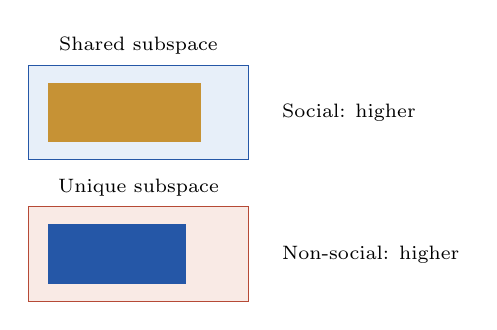
\begin{tikzpicture}[>=Latex]
      \draw[fill=softblue, draw=accentblue] (0,0) rectangle (2.8,1.2);
      \draw[fill=softred, draw=accentred] (0,-1.8) rectangle (2.8,-0.6);
      \fill[accentgold] (0.25,0.22) rectangle (2.2,0.98);
      \fill[accentblue] (0.25,-1.58) rectangle (2.0,-0.82);
      \node at (1.4,1.45) {\scriptsize Shared subspace};
      \node at (1.4,-0.35) {\scriptsize Unique subspace};
      \node[anchor=west] at (3.1,0.6) {\scriptsize Social: higher};
      \node[anchor=west] at (3.1,-1.2) {\scriptsize Non-social: higher};
    \end{tikzpicture}
    \end{center}
  \end{column}
\end{columns}
\end{frame}

\begin{frame}{Result 5b: mutual interaction strengthens the shared subspace}
\begin{columns}[T]
  \begin{column}{0.48\textwidth}
    \begin{itemize}
      \item More \textbf{mutual} social interaction is associated with more shared variance.
      \item Aggressive or antagonistic pairs often show especially strong coupling.
      \item The authors suggest that high-attention interaction may intensify cross-brain coupling.
    \end{itemize}
  \end{column}
  \begin{column}{0.46\textwidth}
    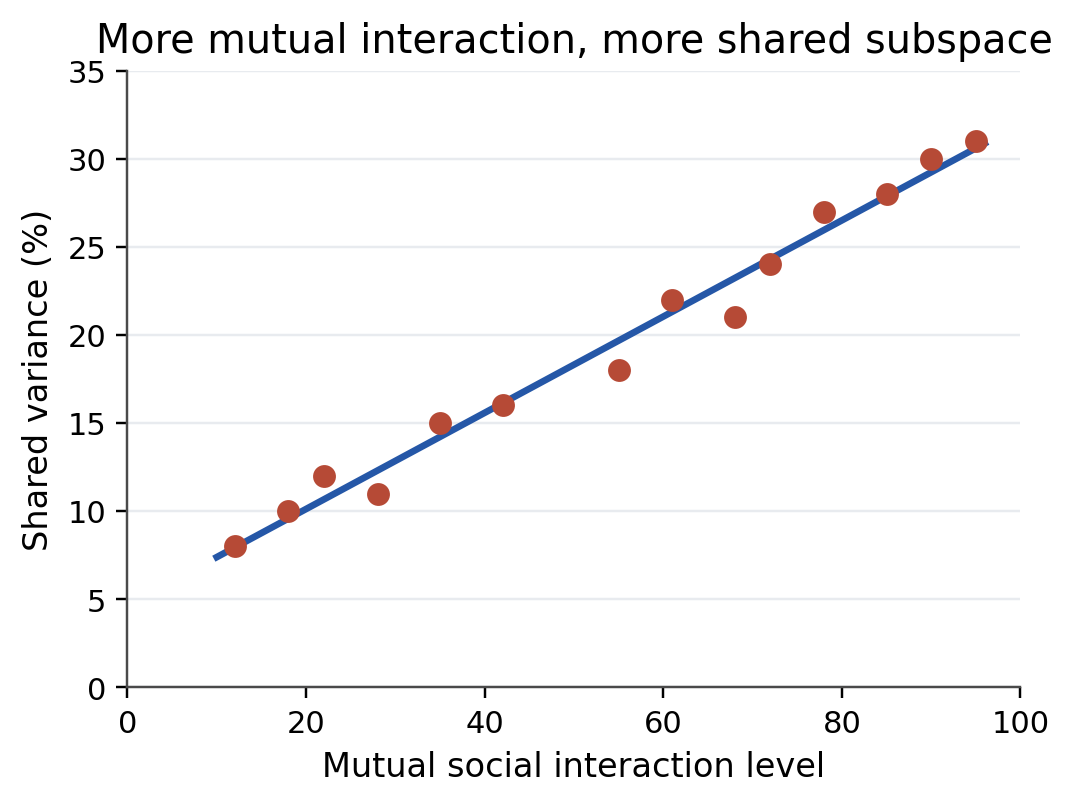
\includegraphics[width=\linewidth]{figures/mutual_interaction_trend.png}
  \end{column}
\end{columns}
\vspace{0.1em}
{\scriptsize The upward trend summarizes the reported positive association between mutual social interaction and GABAergic shared variance.}
\end{frame}

\begin{frame}{Result 6: shared dynamics are not just coordinated behavior}
\begin{columns}[T]
  \begin{column}{0.48\textwidth}
    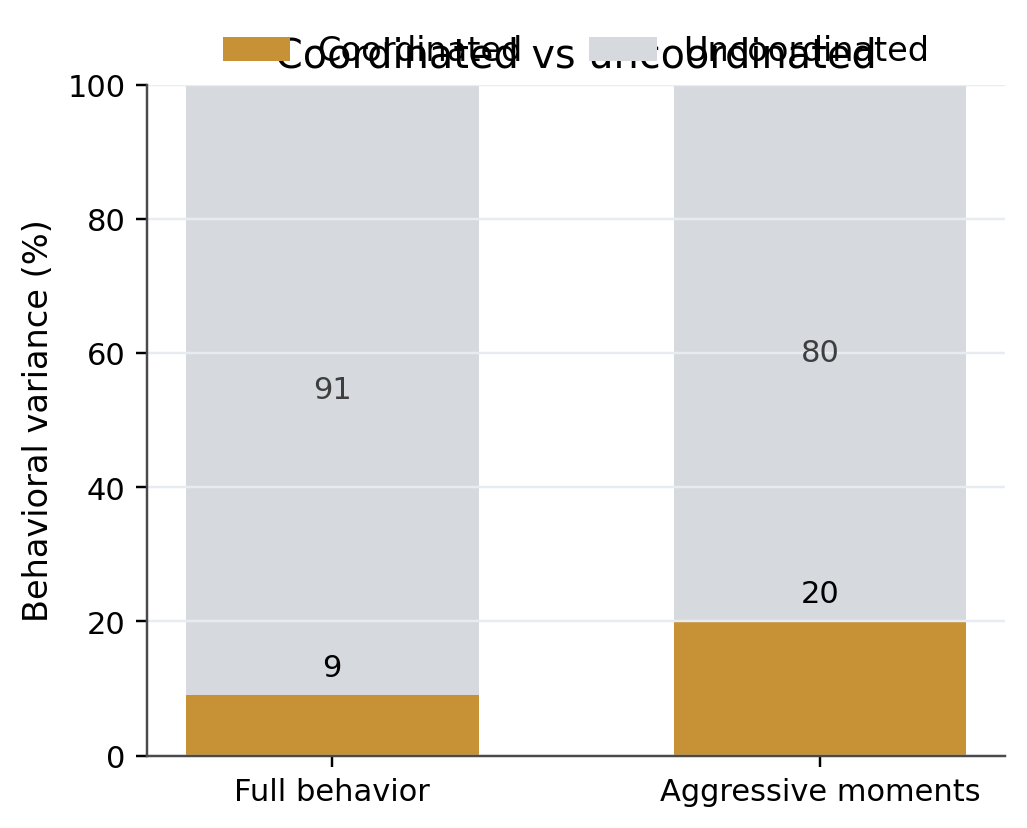
\includegraphics[width=\linewidth]{figures/coordinated_vs_uncoordinated.png}
  \end{column}
  \begin{column}{0.46\textwidth}
    \begin{itemize}
      \item Across 27 pairs, coordinated dimensions explain only about \textbf{9\%} of total behavioral variance.
      \item Even during aggressive interaction, coordinated dimensions explain only about \textbf{20\%}.
      \item So the shared neural subspace also reflects \textbf{uncoordinated but socially linked} behavior.
    \end{itemize}
  \end{column}
\end{columns}
\papersource
\end{frame}

\begin{frame}{Attack versus escape is the key intuition}
\begin{columns}[T]
  \begin{column}{0.52\textwidth}
    \begin{center}
    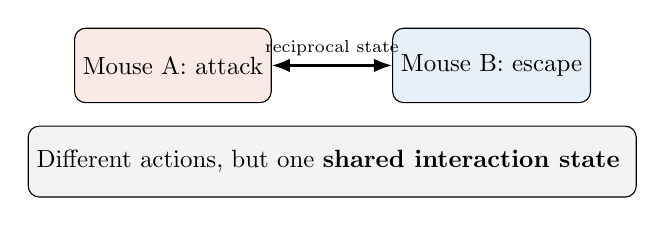
\begin{tikzpicture}[>=Latex, node distance=1.0cm, scale=0.9, transform shape]
      \node[draw, rounded corners, fill=softred, minimum width=2.55cm, minimum height=1.05cm] (a) {Mouse A: attack};
      \node[draw, rounded corners, fill=softblue, right=1.7cm of a, minimum width=2.55cm, minimum height=1.05cm] (b) {Mouse B: escape};
      \draw[<->, thick] (a) -- node[above] {\scriptsize reciprocal state} (b);
      \node[below=0.85cm of $(a)!0.5!(b)$, draw, rounded corners, fill=softgray, minimum width=6.8cm, minimum height=1.0cm, align=center] {
        Different actions, but one \textbf{shared interaction state}
      };
    \end{tikzpicture}
    \end{center}
  \end{column}
  \begin{column}{0.42\textwidth}
    \begin{alertblock}{Interpretive payoff}
    The paper is not just about behavioral synchrony. It is about a jointly represented dyadic state.
    \end{alertblock}
    \begin{itemize}
      \item not simple mimicry
      \item not same action at the same time
      \item more like a shared social game state
    \end{itemize}
  \end{column}
\end{columns}
\end{frame}

\section{AIResults}
\sectiondivider{AI Results}{Does the same logic appear in artificial agents?}

\begin{frame}{AI result 1: social behavior emerges under social training}
\begin{columns}[T]
  \begin{column}{0.54\textwidth}
    \begin{itemize}
      \item Socially trained chasers gain reward over training.
      \item Collisions increase.
      \item Time keeping the partner in vision also increases.
      \item Non-social agents learn exploration, but not the same social following strategy.
    \end{itemize}
  \end{column}
  \begin{column}{0.40\textwidth}
    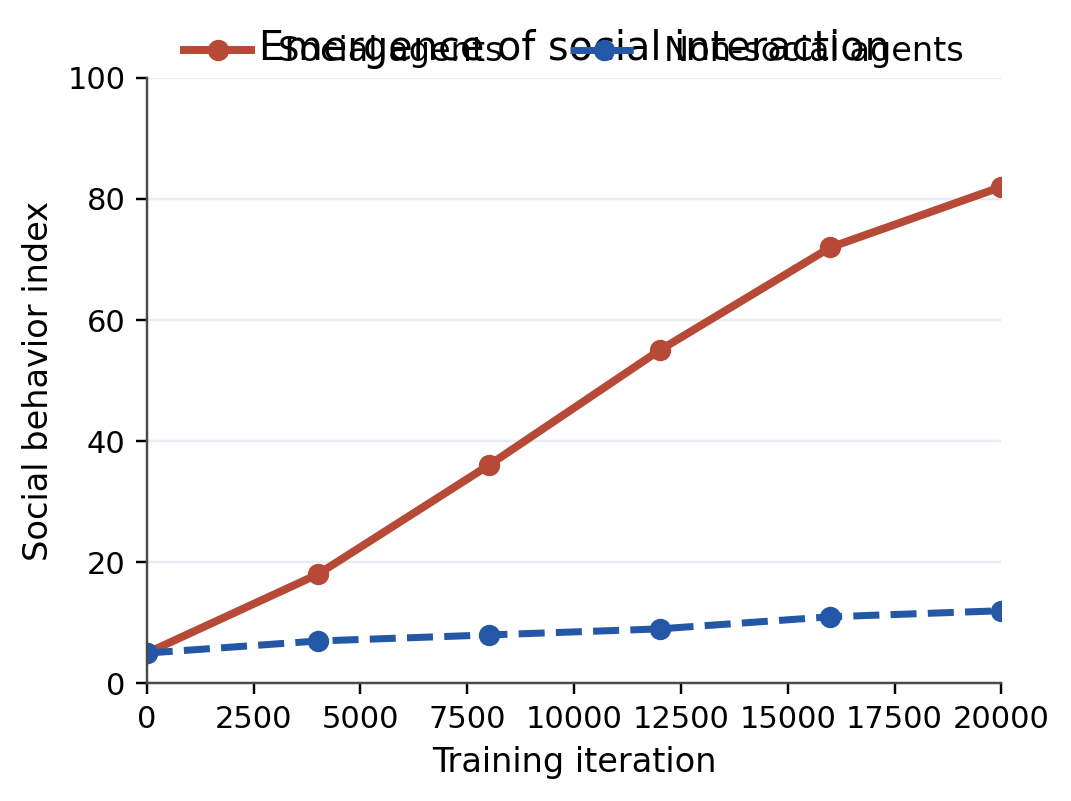
\includegraphics[width=\linewidth]{figures/ai_emergence.png}
  \end{column}
\end{columns}
\vspace{0.1em}
{\scriptsize Curve shape summarizes the training pattern reported in Fig. 5c--h: social behavior rises only in the social environment.}
\end{frame}

\begin{frame}{AI result 2: shared neural dimensions emerge with interaction}
\begin{columns}[T]
  \begin{column}{0.50\textwidth}
    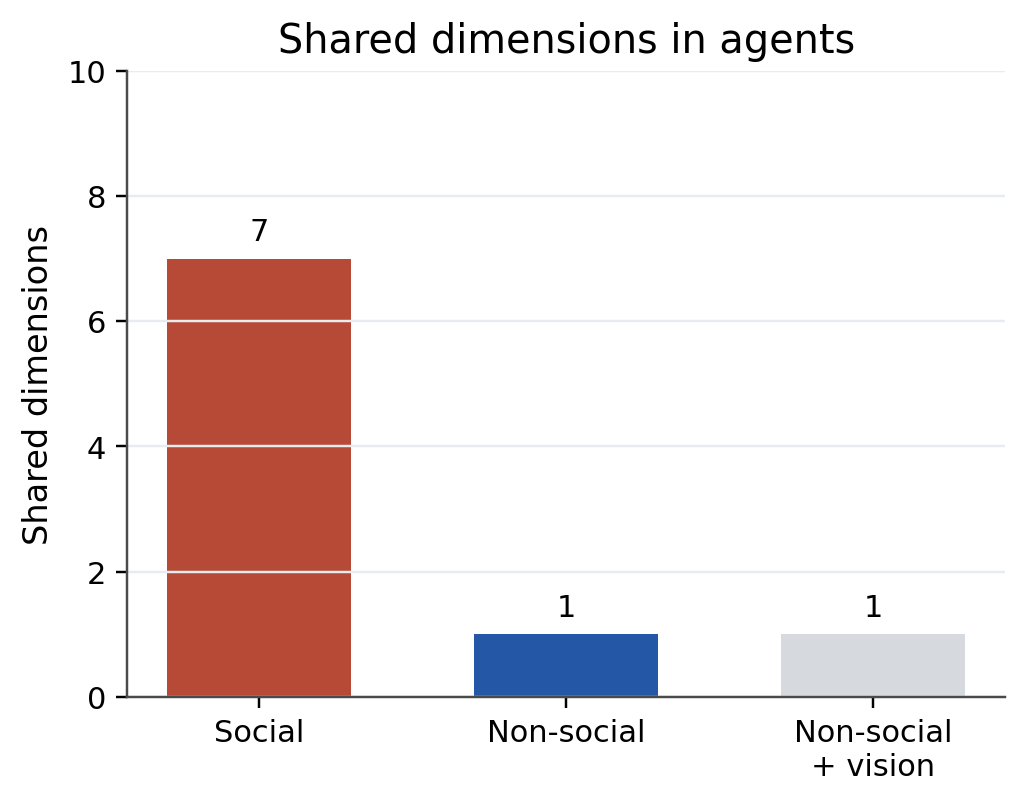
\includegraphics[width=\linewidth]{figures/ai_shared_dimensions.png}
  \end{column}
  \begin{column}{0.44\textwidth}
    \begin{itemize}
      \item Trained social agents have many more shared dimensions.
      \item Giving non-social agents the same or even full visual input does not recreate the shared subspace.
      \item So shared dynamics are not just a consequence of \textbf{seeing the same world}.
    \end{itemize}
  \end{column}
\end{columns}
\vspace{0.1em}
{\scriptsize Relative bar heights summarize the contrast reported in Fig. 6g and Extended Data Fig. 13a.}
\end{frame}

\begin{frame}{AI result 3: partner behavior is represented in social agents}
\begin{columns}[T]
  \begin{column}{0.54\textwidth}
    \begin{itemize}
      \item Social agents' RNN activity can decode:
      \begin{itemize}
        \item collision events,
        \item partner approach,
        \item partner escape.
      \end{itemize}
      \item Non-social agents cannot do this at the same level.
      \item Just like in mice, \textbf{partner representation is enriched in the shared dimensions}.
    \end{itemize}
  \end{column}
  \begin{column}{0.40\textwidth}
    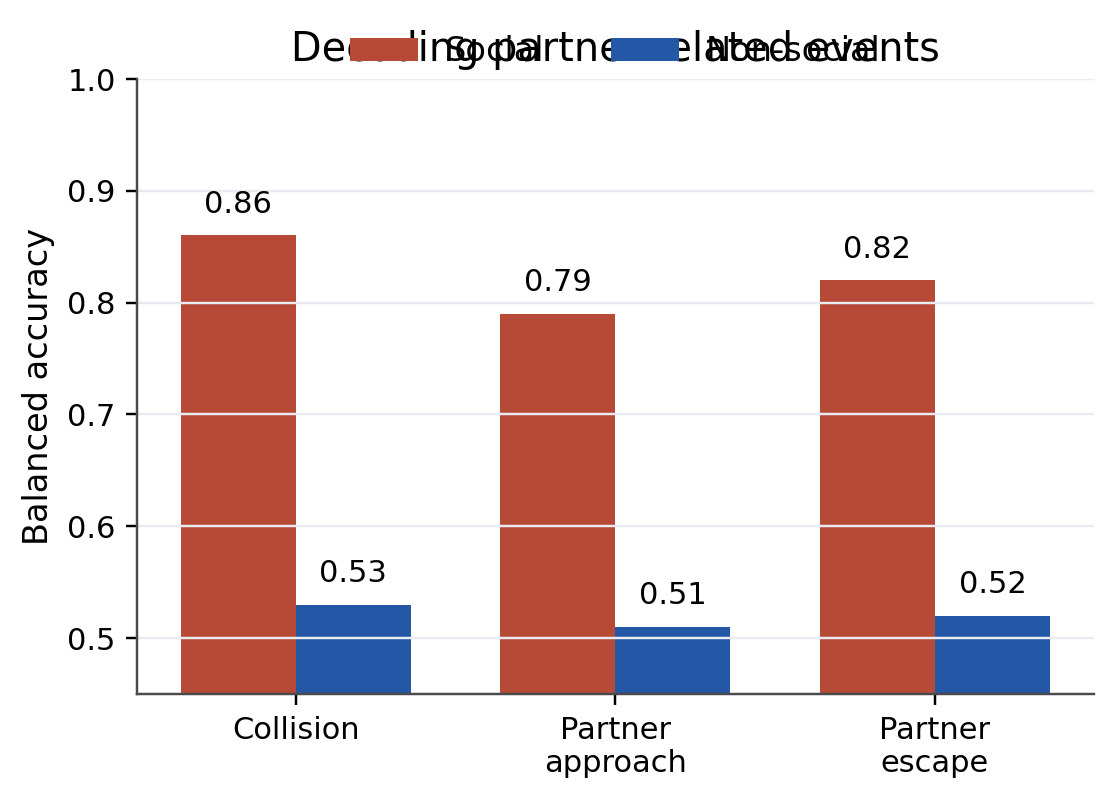
\includegraphics[width=\linewidth]{figures/ai_decoding.png}
  \end{column}
\end{columns}
\end{frame}

\begin{frame}{AI result 4: perturbing shared components reduces social action}
\begin{columns}[T]
  \begin{column}{0.48\textwidth}
    \begin{block}{What they perturb}
    Neural components that strongly contribute to the top shared dimensions.
    \end{block}
    \begin{block}{What happens}
    Social action declines, including a drop in collisions.
    \end{block}
  \end{column}
  \begin{column}{0.46\textwidth}
    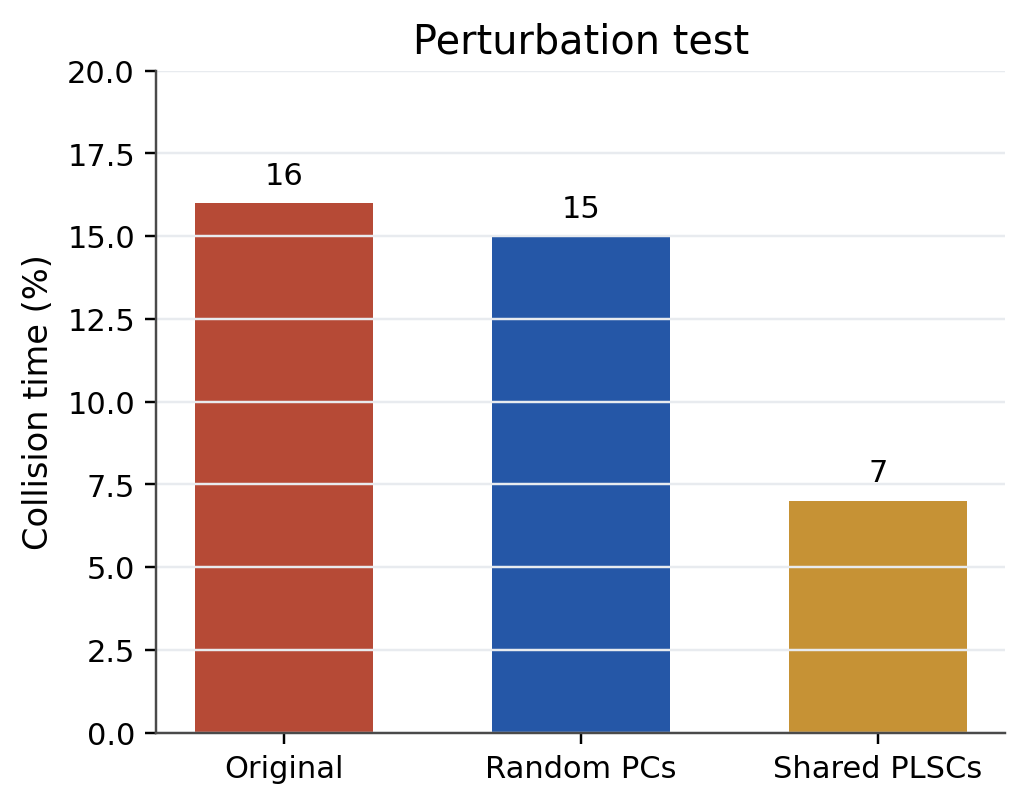
\includegraphics[width=0.9\linewidth]{figures/ai_perturbation.png}
  \end{column}
\end{columns}
\vspace{0.2em}
\begin{alertblock}{Why this is important}
This is the paper's strongest evidence that shared components matter for behavior.
\end{alertblock}
\end{frame}

\begin{frame}{What looks similar across mice and AI?}
\begin{center}
\small
\begin{tabular}{>{\raggedright\arraybackslash}p{0.22\linewidth} >{\raggedright\arraybackslash}p{0.34\linewidth} >{\raggedright\arraybackslash}p{0.34\linewidth}}
\toprule
 & \textbf{Mice} & \textbf{AI agents} \\
\midrule
Shared dimensions emerge? & Yes, during live interaction & Yes, during social training \\
Just same input / same action? & No, behavior controls argue against that & No, shared-input and identical-action controls argue against that \\
Partner representation? & Yes, especially in the shared subspace & Yes, especially in social agents \\
Functional perturbation? & Not directly in vivo & Yes, social behavior drops after perturbation \\
Main limitation & Mostly correlational & Simplified task and architecture \\
\bottomrule
\end{tabular}
\end{center}
\end{frame}

\section{Interpretation}
\sectiondivider{Interpretation}{Should we buy the authors' story?}

\begin{frame}{Authors' interpretation}
\begin{block}{Main claim}
Shared neural dynamics are a \textbf{fundamental and generalizable feature} of interacting neural systems in both biological and artificial agents.
\end{block}
\vspace{0.4em}
\begin{itemize}
  \item Two interacting individuals should be treated as one integrated system.
  \item GABAergic neurons play a special role in the biological case.
  \item The shared subspace is behaviorally meaningful, not just mathematical structure.
  \item AI results provide functional support for the importance of shared components.
\end{itemize}
\end{frame}

\begin{frame}{Why I find the paper convincing}
\begin{enumerate}
  \item \textbf{Strong controls}: separation, phase randomization, cross-pairing, pre-whitening, and behavior-space analyses
  \item \textbf{Cell-type specificity}: the story is not only ``dmPFC synchronizes''
  \item \textbf{High-dimensional framing}: the paper moves beyond average correlation
  \item \textbf{AI perturbation}: shared components are tied to social behavior, at least in the artificial system
\end{enumerate}
\end{frame}

\begin{frame}{Why I am still cautious}
\begin{columns}[T]
  \begin{column}{0.48\textwidth}
    \begin{alertblock}{Causality gap in mice}
    The mouse evidence is still largely correlational and computational.
    \end{alertblock}
    \begin{itemize}
      \item We do not yet know whether shared dynamics are a cause or a consequence of social interaction.
      \item The paper does not directly manipulate the relevant mouse ensembles in vivo.
    \end{itemize}
  \end{column}
  \begin{column}{0.48\textwidth}
    \begin{alertblock}{The AI analogy has limits}
    AI agents are not mouse brains.
    \end{alertblock}
    \begin{itemize}
      \item Different architecture
      \item Different learning rules
      \item Different motivational structure
    \end{itemize}
  \end{column}
\end{columns}
\end{frame}

\begin{frame}{Four limitations I would say out loud in class}
\begin{enumerate}
  \item \textbf{Aggression-heavy context}: some of the strongest shared signals appear in aggressive, high-attention interaction.
  \item \textbf{One-region window}: dmPFC is only one piece of the social brain network.
  \item \textbf{Interpretability problem}: a statistically meaningful PLSC dimension does not automatically have a clean biological meaning.
  \item \textbf{Generalization risk}: cooperation, bonding, empathy, or teaching may show different dynamics.
\end{enumerate}
\end{frame}

\begin{frame}{My bottom line}
\begin{columns}[T]
  \begin{column}{0.45\textwidth}
    \begin{block}{I buy}
    \begin{itemize}
      \item Interacting brains really do show shared structure
      \item GABAergic neurons seem especially important
      \item The effect is not reducible to simple motor coordination
    \end{itemize}
    \end{block}
  \end{column}
  \begin{column}{0.50\textwidth}
    \begin{alertblock}{I do not fully buy}
    \begin{itemize}
      \item that the paper has already proven a universal principle,
      \item that AI results map directly onto biological mechanism,
      \item or that attention, arousal, and social computation are fully separated here.
    \end{itemize}
    \end{alertblock}
  \end{column}
\end{columns}
\end{frame}

\section{Extension}
\sectiondivider{Extension}{How would I redesign or extend the work?}

\begin{frame}{Redesign 1: add causal manipulation in mice}
\begin{columns}[T]
  \begin{column}{0.54\textwidth}
    \begin{itemize}
      \item Target \textbf{social-responsive GABAergic ensembles} with optogenetic or chemogenetic manipulation.
      \item Ideally use a closed-loop design that intervenes when a high shared state is detected.
      \item Directly measure:
      \begin{itemize}
        \item social interaction probability,
        \item inter-brain correlation,
        \item shared subspace size.
      \end{itemize}
    \end{itemize}
  \end{column}
  \begin{column}{0.40\textwidth}
    \begin{center}
    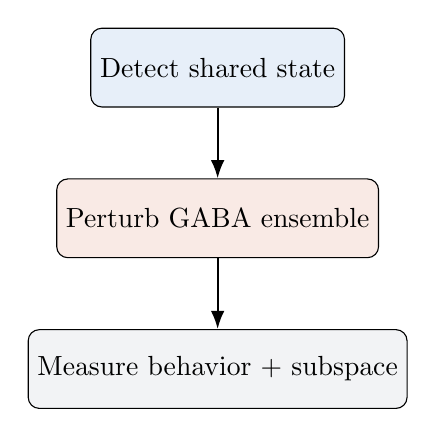
\begin{tikzpicture}[>=Latex]
      \node[draw, rounded corners, fill=softblue, minimum width=2.8cm, minimum height=1cm] (detect) {Detect shared state};
      \node[draw, rounded corners, fill=softred, below=0.9cm of detect, minimum width=2.8cm, minimum height=1cm] (perturb) {Perturb GABA ensemble};
      \node[draw, rounded corners, fill=softgray, below=0.9cm of perturb, minimum width=3.4cm, minimum height=1cm] (measure) {Measure behavior + subspace};
      \draw[->, thick] (detect) -- (perturb);
      \draw[->, thick] (perturb) -- (measure);
    \end{tikzpicture}
    \end{center}
  \end{column}
\end{columns}
\end{frame}

\begin{frame}{Redesign 2: compare different social contexts}
\begin{columns}[T]
  \begin{column}{0.47\textwidth}
    \begin{block}{Current concern}
    The strongest shared signals are closely tied to aggression and close mutual attention.
    \end{block}
  \end{column}
  \begin{column}{0.47\textwidth}
    \begin{block}{Better design}
    \begin{itemize}
      \item cooperation
      \item mating
      \item parent-offspring interaction
      \item familiar versus unfamiliar pairs
      \item dominance hierarchy
    \end{itemize}
    \end{block}
  \end{column}
\end{columns}
\vspace{0.4em}
\begin{alertblock}{Question}
Is shared neural dynamics a general feature of all social interaction, or especially strong in high-arousal and high-attention interaction?
\end{alertblock}
\end{frame}

\begin{frame}{Redesign 3: make the task more neuroeconomic}
\begin{itemize}
  \item The current mouse setting is socially rich, but not explicitly structured as a strategic game.
  \item To connect more directly to neuroeconomics, I would add:
\end{itemize}
\begin{center}
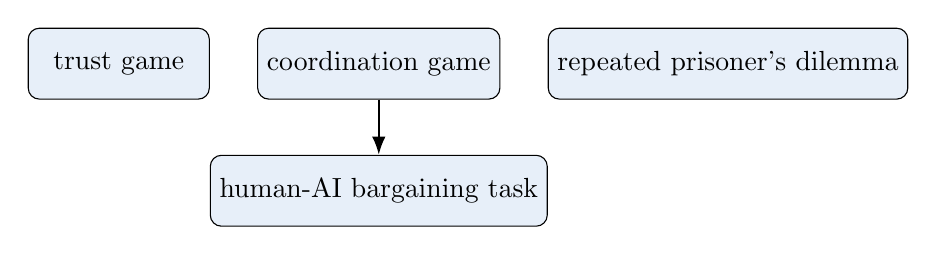
\begin{tikzpicture}[>=Latex, node distance=0.7cm]
  \node[draw, rounded corners, fill=softblue, minimum width=2.3cm, minimum height=0.9cm] (t1) {trust game};
  \node[draw, rounded corners, fill=softblue, right=0.6cm of t1, minimum width=2.3cm, minimum height=0.9cm] (t2) {coordination game};
  \node[draw, rounded corners, fill=softblue, right=0.6cm of t2, minimum width=2.3cm, minimum height=0.9cm] (t3) {repeated prisoner's dilemma};
  \node[draw, rounded corners, fill=softblue, below=0.7cm of t2, minimum width=2.8cm, minimum height=0.9cm] (t4) {human-AI bargaining task};
  \draw[->, thick] (t2) -- (t4);
\end{tikzpicture}
\end{center}
\vspace{0.3em}
\begin{block}{Key question}
Do cooperation, betrayal, trust building, and trust collapse create different shared neural states?
\end{block}
\end{frame}

\begin{frame}{Proposed new experiment: shared neural dynamics in a trust game}
\begin{columns}[T]
  \begin{column}{0.55\textwidth}
    \begin{itemize}
      \item Participants: human-human pairs
      \item Task: \textbf{repeated trust game}
      \item Recording: EEG hyperscanning or fNIRS hyperscanning
      \item Conditions:
      \begin{itemize}
        \item human-human
        \item human-AI
        \item human-random-bot
      \end{itemize}
    \end{itemize}
  \end{column}
  \begin{column}{0.39\textwidth}
    \begin{center}
    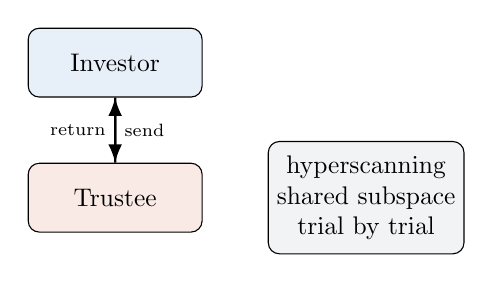
\begin{tikzpicture}[>=Latex, node distance=0.9cm, scale=0.92, transform shape]
      \node[draw, rounded corners, fill=softblue, minimum width=2.4cm, minimum height=0.95cm] (i) {Investor};
      \node[draw, rounded corners, fill=softred, below=0.9cm of i, minimum width=2.4cm, minimum height=0.95cm] (t) {Trustee};
      \draw[->, thick] (i) -- node[right] {\scriptsize send} (t);
      \draw[->, thick] (t) -- node[left] {\scriptsize return} (i);
      \node[draw, rounded corners, fill=softgray, right=0.9cm of t, minimum width=2.5cm, minimum height=1.55cm, align=center] {
        hyperscanning\\
        shared subspace\\
        trial by trial
      };
    \end{tikzpicture}
    \end{center}
  \end{column}
\end{columns}
\end{frame}

\begin{frame}{Predictions for the trust-game extension}
\begin{enumerate}
  \item High-trust pairs should show stronger inter-brain synchrony or shared subspace structure.
  \item As trust builds over rounds, the shared subspace should become stronger or more stable.
  \item After betrayal, the shared subspace may weaken or reorganize.
  \item Current shared dynamics may predict next-round cooperation.
  \item Human-AI interaction may sit between human-human and random-bot conditions.
\end{enumerate}
\end{frame}

\begin{frame}{Why this is genuinely neuroeconomics}
\begin{columns}[T]
  \begin{column}{0.48\textwidth}
    \begin{block}{Behavioral concepts}
    \begin{itemize}
      \item trust
      \item reciprocity
      \item strategic uncertainty
      \item belief updating
      \item cooperation breakdown
    \end{itemize}
    \end{block}
  \end{column}
  \begin{column}{0.48\textwidth}
    \begin{block}{Neural concepts}
    \begin{itemize}
      \item shared subspace
      \item partner representation
      \item coupled decision systems
      \item prediction of future actions
    \end{itemize}
    \end{block}
  \end{column}
\end{columns}
\vspace{0.4em}
\begin{alertblock}{Take-home extension}
Trust may not be only a preference inside one brain. It may also be a \textbf{dyadic neural process} distributed across two interacting agents.
\end{alertblock}
\end{frame}

\section{Discussion}
\sectiondivider{Discussion}{What should the class talk about?}

\begin{frame}{Discussion questions}
\begin{enumerate}
  \item Are shared neural dynamics a \textbf{cause} of social interaction or a \textbf{consequence} of it?
  \item Does GABAergic dominance really reflect social coding, or could it be closer to attention or arousal gating?
  \item Would cooperation and aggression generate different kinds of shared subspace?
  \item How far can we compare shared dynamics in humans and AI?
  \item Can the current shared state predict the next action: attack, escape, cooperate, or defect?
\end{enumerate}
\end{frame}

\begin{frame}{Final takeaway}
\begin{alertblock}{If you remember only one thing}
The paper's biggest contribution is to treat social interaction not as one brain reacting to another individual, but as two interacting agents forming a joint neural dynamic system.
\end{alertblock}
\vspace{0.5em}
\begin{itemize}
  \item In mice, GABAergic dmPFC neurons contain a larger shared subspace.
  \item Shared dynamics are not reducible to simple behavioral coordination.
  \item In AI, shared components emerge with interaction and matter for social action.
  \item For neuroeconomics, strategic interaction may be neurally \textbf{coupled}, not isolated.
\end{itemize}
\end{frame}

\begin{frame}{Reference}
\small
\begin{thebibliography}{9}
\bibitem{zhang2025}
Zhang, X., Phi, N., Li, Q., Gorzek, R., Zwingenberger, N., Huang, S., Zhou, J. L., Kingsbury, L., Raam, T., Wu, Y. E., Wei, D., Kao, J. C., \& Hong, W. (2025).\\
\textit{Inter-brain neural dynamics in biological and artificial intelligence systems}.\\
Nature, 645, 991--1001. DOI: 10.1038/s41586-025-09196-4
\end{thebibliography}
\end{frame}

\appendix
\section{Appendix}
\sectiondivider{Appendix}{Extra support slides for Q\&A}

\begin{frame}{Appendix: useful numeric anchors}
\begin{itemize}
  \item 9,006 glutamatergic neurons from 13 mouse pairs
  \item 3,331 GABAergic neurons from 14 mouse pairs
  \item Mice spent about 49\% of time in active behavior
  \item About 48\% of active behavior was social
  \item About 45\% of GABAergic neurons were social-responsive
  \item About 10\% of glutamatergic neurons were social-responsive
  \item Shared variance was roughly 30\% in GABAergic populations versus 5\% in glutamatergic populations
\end{itemize}
\papersource
\end{frame}

\begin{frame}{Appendix: why the coordinated-behavior control is so important}
\begin{columns}[T]
  \begin{column}{0.48\textwidth}
    \begin{block}{Without this control}
    A critic can always say:
    \begin{itemize}
      \item the animals simply move together,
      \item stop together,
      \item or enter the same high-arousal state.
    \end{itemize}
    \end{block}
  \end{column}
  \begin{column}{0.48\textwidth}
    \begin{alertblock}{With this control}
    The authors can argue more strongly that:
    \begin{itemize}
      \item partner-specific information enters the shared subspace,
      \item especially through complementary rather than identical actions.
    \end{itemize}
    \end{alertblock}
  \end{column}
\end{columns}
\end{frame}

\begin{frame}{Appendix: one clean sentence about PLSC}
\begin{block}{Presentation-friendly definition}
PLSC finds the cross-brain neural dimensions that \textbf{co-vary the most}, allowing the authors to separate what is \textbf{shared across two interacting agents} from what remains \textbf{unique to each individual}.
\end{block}
\vspace{0.6em}
\begin{itemize}
  \item This is a useful sentence to say if the instructor asks about the method.
  \item Then you can add: the shared subspace is more social, whereas the unique subspace is more self-specific.
\end{itemize}
\end{frame}

\begin{frame}{Appendix: how to answer ``Why is this neuroeconomics?''}
\begin{enumerate}
  \item The core issue is \textbf{interactive decision systems}, not static social cue processing.
  \item Self and other are mutually endogenous, just like in strategic models.
  \item The paper connects naturally to trust, cooperation, competition, and reciprocity.
  \item It offers a neural version of \textbf{best-response coupling}.
\end{enumerate}
\end{frame}

\begin{frame}{Appendix: what about humans?}
\begin{itemize}
  \item The most realistic human path is EEG or fNIRS hyperscanning, not cell-type recording.
  \item The main challenge is not whether synchrony exists, but whether we can build a convincing \textbf{shared versus unique subspace} analysis tied to behavior.
  \item Human studies are especially well suited for:
  \begin{itemize}
    \item trust games,
    \item bargaining,
    \item joint problem solving,
    \item human-AI collaboration.
  \end{itemize}
\end{itemize}
\end{frame}

\end{document}
